\headline{{\textbf{\Large\sffamily The Top Chop:}}\\
{\textbf{\large\sffamily The Tree of the Month Competition}}}
\phantomsection
\label{2026-01-totm}
\noindent
Our first meeting of 2026 stripped away the holiday decorations to reveal the raw beauty of winter.
The theme, \textit{``Naked tree, Elm''}, challenged members to showcase the intricate ramification and delicate structure of their deciduous trees without the camouflage of foliage.
The benches were filled with impressive winter silhouettes, offering a masterclass in fine wiring and structural development.

\medskip
\noindent
For our new members, here is a reminder of how we judge our trees.
Attending members vote on every tree except their own to maintain a fair balance.
Each tree is awarded between 1 (lowest) and 3 (highest) points across four key categories: \textbf{trunk and branch structure}, \textbf{ramification and twigging} (vital for the winter theme), \textbf{pot suitability}, and \textbf{overall presentation}.

\noindent
Total scores are calculated by summing these points.
Unlike the December festive round, January’s results are recorded for the 2026 annual league table.
For a deep dive into the scoring system, please see the \textbf{November 2025 newsletter}.

\medskip
\topic{General Tree of the Month}
\noindent
The General category displayed some truly mature specimens, with the cork-bark varieties particularly catching the eye of the voters.

\begin{enumerate}
    \item \textbf{Tony Ulatowski}'s Cork Bark Elm (\textit{`Ulmus parvifolia 'Corticosa''}) --- 150 points.
    A stunning display of textured bark and balanced structure that dominated the scoring.
    \item \textbf{Kenny Chan}'s Cork Bark Elm (\textit{`Ulmus parvifolia 'Corticosa''}) --- 144 points.
    \item \textbf{Terry Wilson}'s English Elm (\textit{`Ulmus procera'}) --- 132 points.
    \item \textbf{Tina Todd}'s Cork Bark Elm (\textit{`Ulmus parvifolia 'Corticosa''}) --- 125 points.
    \item \textbf{David Fishwick}'s English Elm (\textit{`Ulmus procera'}) --- 118 points.
    \item \textbf{Mark Pittman}'s Elm (\textit{`Ulmus'}) --- 91 points.
\end{enumerate}

\noindent
Congratulations to \textbf{Tony Ulatowski} for taking the first top spot of the new year!

\medskip
\topic{Novice Tree of the Month}
\noindent
Our Novice section showed great promise, with members bringing in varied species that highlighted the diversity within the deciduous category.

\begin{enumerate}
    \item \textbf{Victoria Miquel}'s Plum (\textit{`Prunus'}) --- 94 points.
    An elegant silhouette that was made even more feminine by the presence of delicate flowers.
    \item \textbf{Laura Shantonas}'s Ledebouria (\textit{`Ledebouria'}) --- 61 points.
\end{enumerate}

\noindent
Well done to our Novice winner, \textbf{Victoria Miquel}, for a well\--deserved victory!

%\medskip
%\noindent
%The evening also served as a moment to celebrate the champions of the previous year.
%The trophies for the 2025 Overall Tree of the Month Competition were awarded to our top\--performing members across the entire season.
%In the Novice category, \textbf{Martin Redfern} took the top spot; though he was unable to attend the meeting, his prize was presented during the MEP.
%In the General category, \textbf{Brendan Gibbs} emerged as the overall winner and was presented with the trophy by Nick Ulatowski.

\medskip
\noindent
We also celebrated our 2025 champions: \textbf{Martin Redfern} won the Novice category (presented at the MEP), while \textbf{Brendan Gibbs} took the General class trophy, presented by Tony Ulatowski.

\vspace*{-0.5em}
\begin{center}
    $\cdots$
\end{center}
\vspace*{-0.5em}

\noindent
Starting the year with elms allowed us to appreciate the hard work put into the ``bones'' of our trees during the dormant season.
As we move into February, our theme shifts toward classical aesthetics: \textit{``Formal / Informal styles''}.
It will be a great opportunity to discuss line, balance, and the traditional rules of bonsai design.

See you all in February!

\noindent
\begin{center}
    \begin{minipage}[b]{.4\columnwidth}
        
\includegraphics[angle=0,origin=c,width=1.0\textwidth]{2026_01/res/2601_totm_winner1}
    \end{minipage}\quad
    \begin{minipage}[b]{.4\columnwidth}
        
\includegraphics[angle=0,origin=c,width=1.0\textwidth]{2026_01/res/2601_totm_winner2}
    \end{minipage}
    \centerline{\textit{Tony Ulatowski and Victoria Miquel receive their General}}
    \centerline{\textit{and Novice TOTM certificates.}}
\end{center}

\noindent
\begin{center}
    \begin{minipage}[b]{0.45\textwidth}
        \quad
\includegraphics[angle=0,origin=c,width=0.9\textwidth]{2026_01/res/2601_totm_brendan_wins}
        \centerline{\emph{Brendan Gibbs composedly accepts the TOTM `25 award.}}
    \end{minipage}
\end{center}
\closearticle
\clearpage

\topic{January 2026 General TOTM Trees}

\begin{minipage}[b]{.45\textwidth}
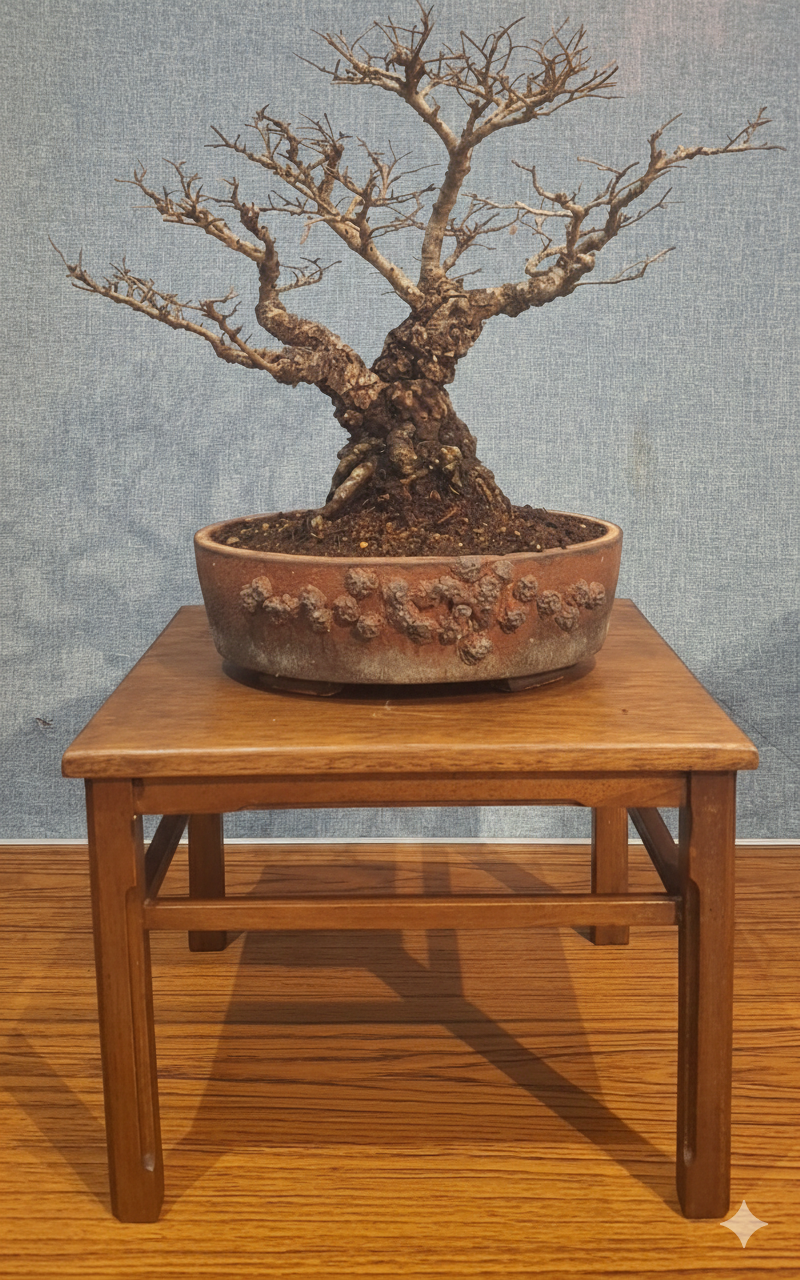
\includegraphics[angle=0,origin=c,width=1.0\textwidth]{2026_01/res/2601_totm_1_ulatowski}
\centerline{\emph{Tony Ulatowski's Cork Bark Elm.}}
\end{minipage}
\medskip

\begin{minipage}[b]{.45\textwidth}
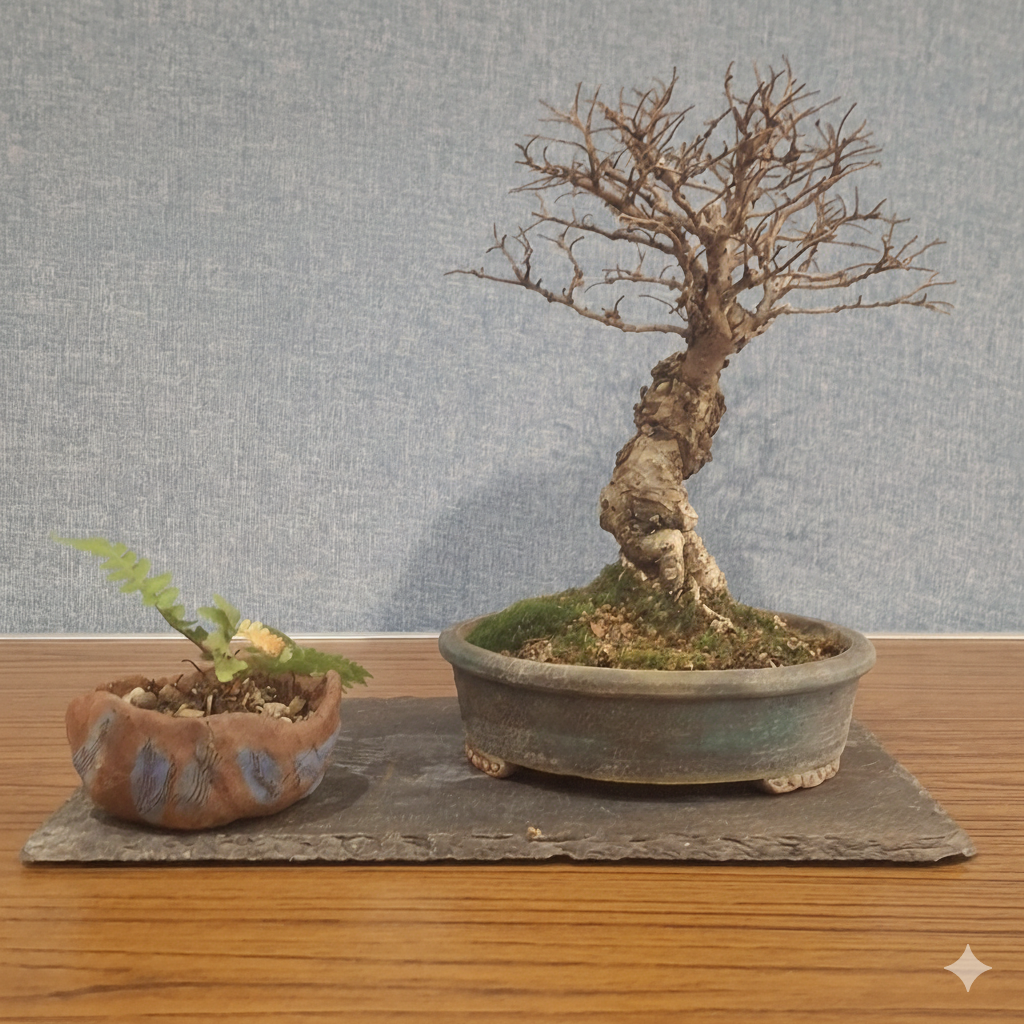
\includegraphics[angle=0,origin=c,width=1.0\textwidth]{2026_01/res/2601_totm_2_chan}
\centerline{\emph{
Kenny Chan's Cork Bark Elm.}}
\end{minipage}
\medskip

\vfill
\columnbreak

\topic{\textcolor{white}{space}}

\begin{minipage}[b]{.45\textwidth}
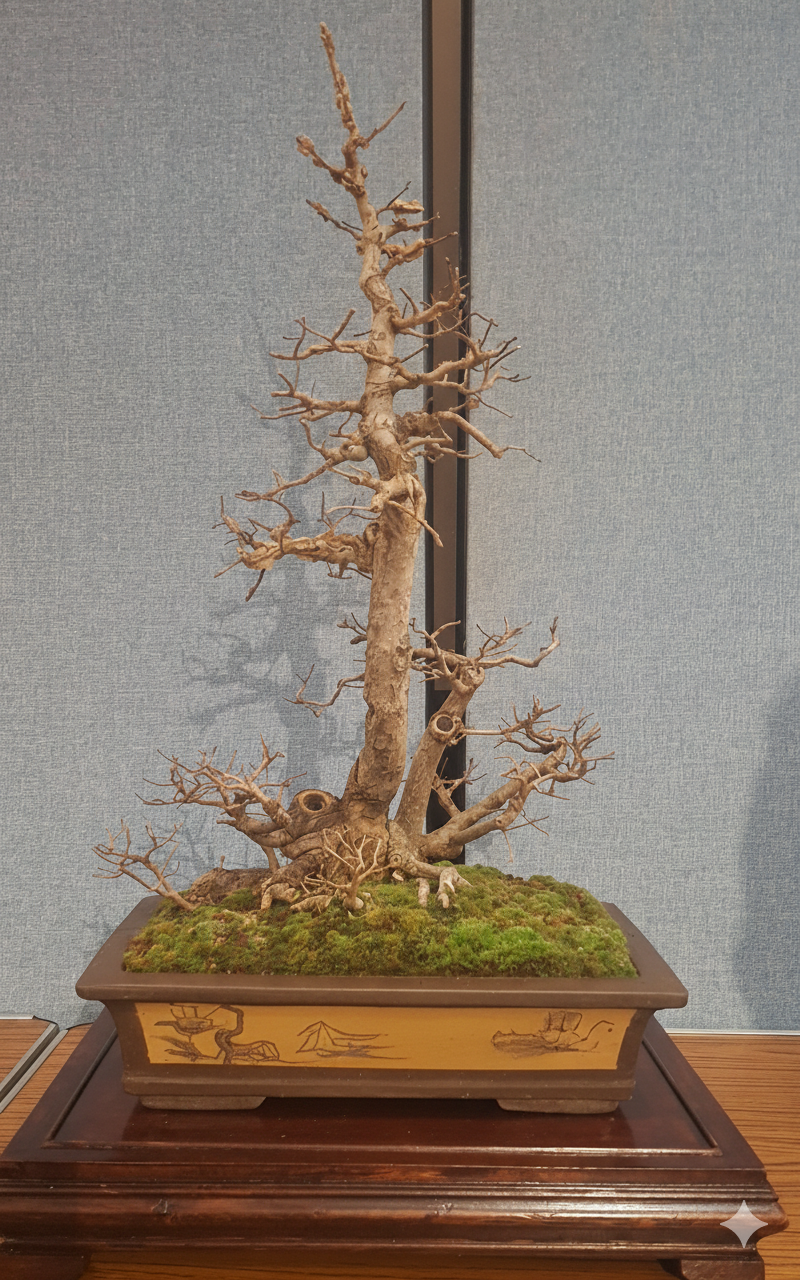
\includegraphics[angle=0,origin=c,width=1.0\textwidth]{2026_01/res/2601_totm_3_wilson}
\centerline{\emph{Terry Wilson's English Elm.}}
\end{minipage}
\medskip

\begin{minipage}[b]{.45\textwidth}
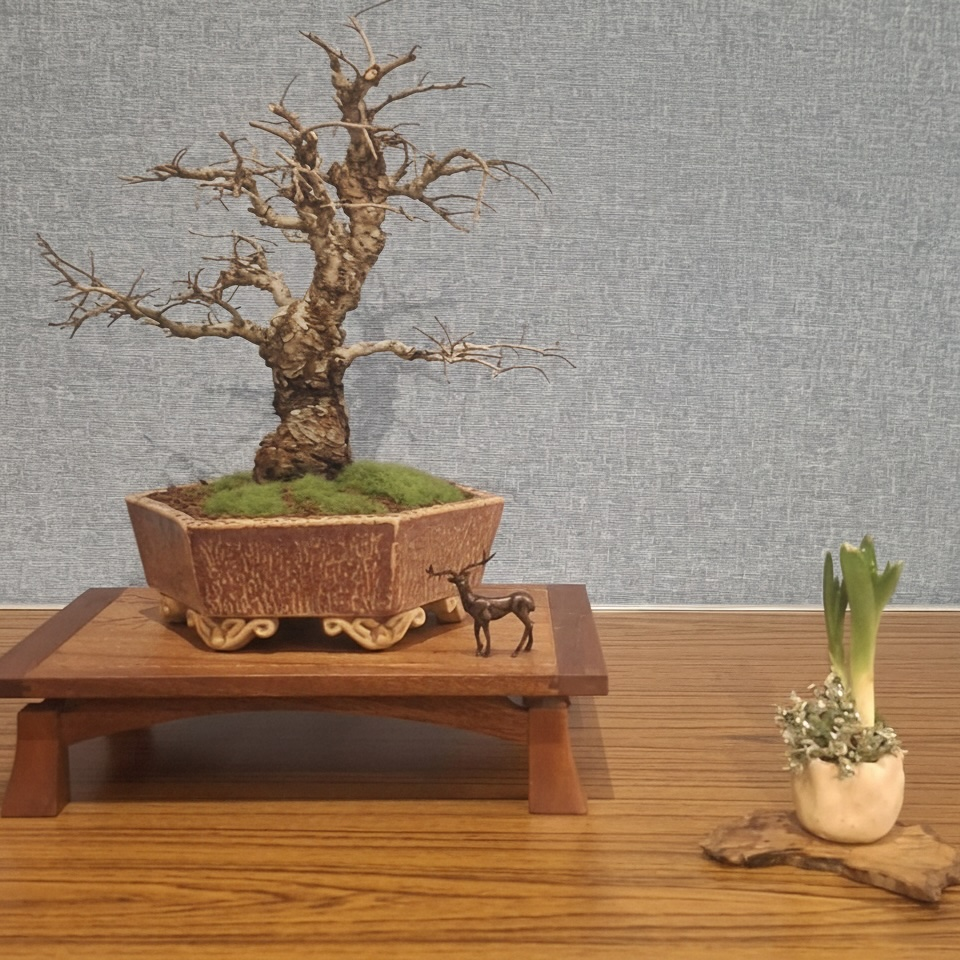
\includegraphics[angle=0,origin=c,width=1.0\textwidth]{2026_01/res/2601_totm_4_todd}
\centerline{\emph{Tina Todd's Cork Bark Elm.}}
\end{minipage}
\medskip

\vfill
\columnbreak

\begin{minipage}[b]{.45\textwidth}
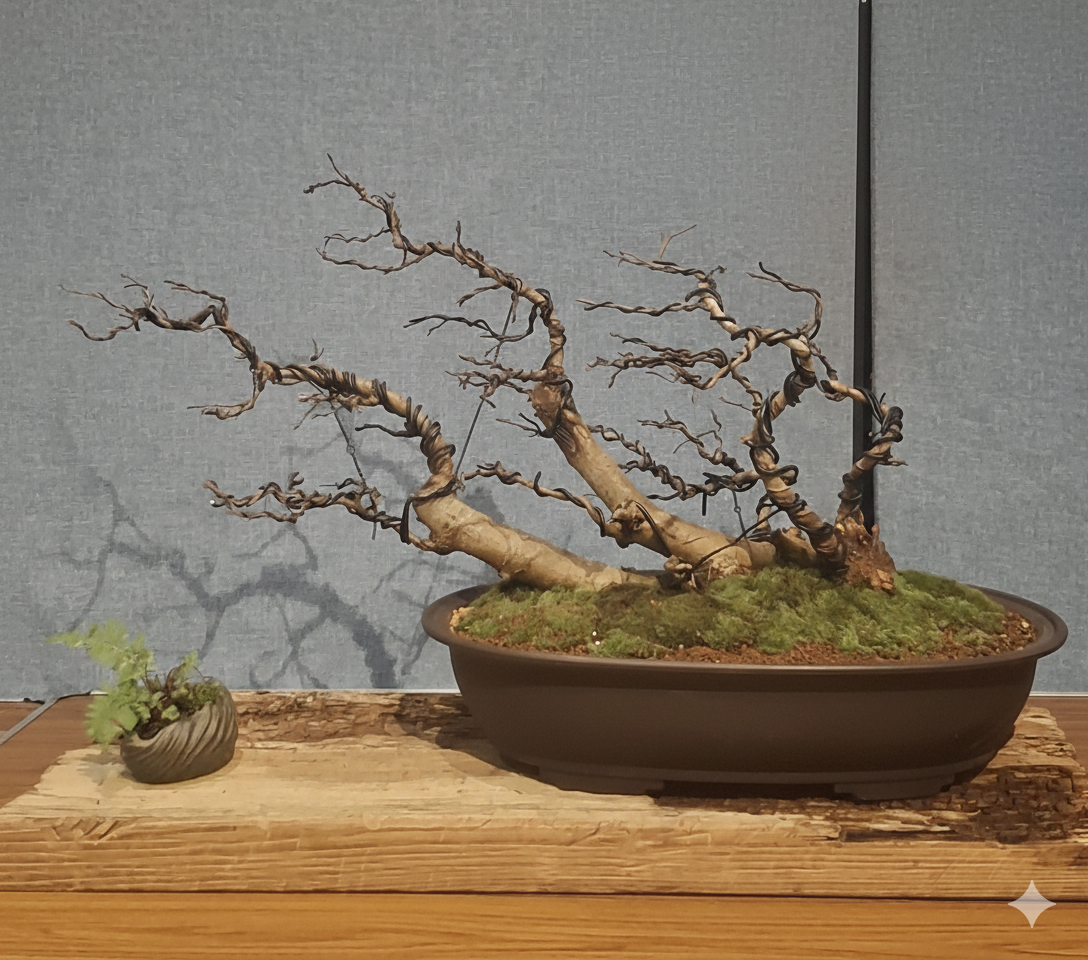
\includegraphics[angle=0,origin=c,width=1.0\textwidth]{2026_01/res/2601_totm_5_fishwick}
\centerline{\emph{David Fishwick's English Elm.}}
\end{minipage}
\medskip

\vfill
\topic{January 2026 Novice TOTM Trees}

\begin{minipage}[b]{.45\textwidth}
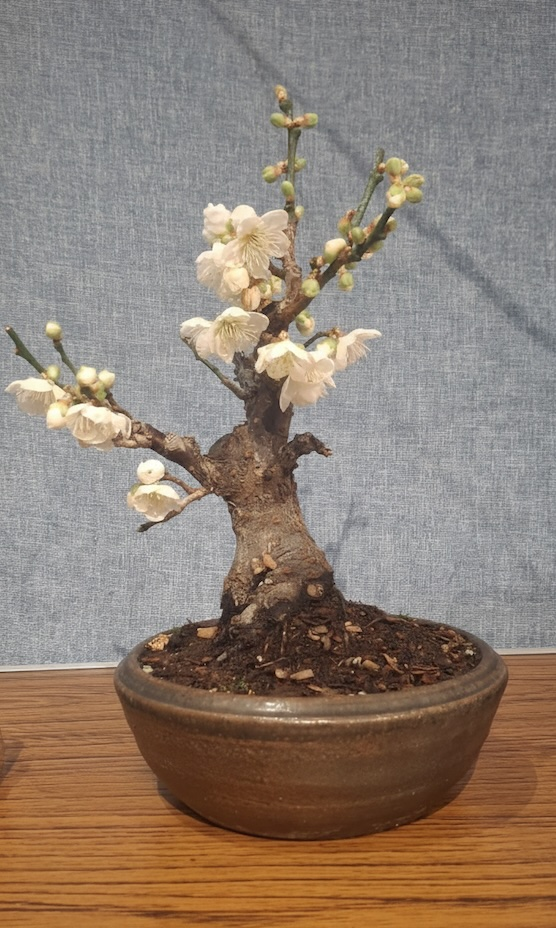
\includegraphics[angle=0,origin=c,width=1.0\textwidth]{2026_01/res/2601_totm_nov_victoria}
\centerline{\emph{Victoria Miquel's Plum.}}
\end{minipage}
\medskip

\vfill
\columnbreak

\begin{minipage}[b]{.45\textwidth}
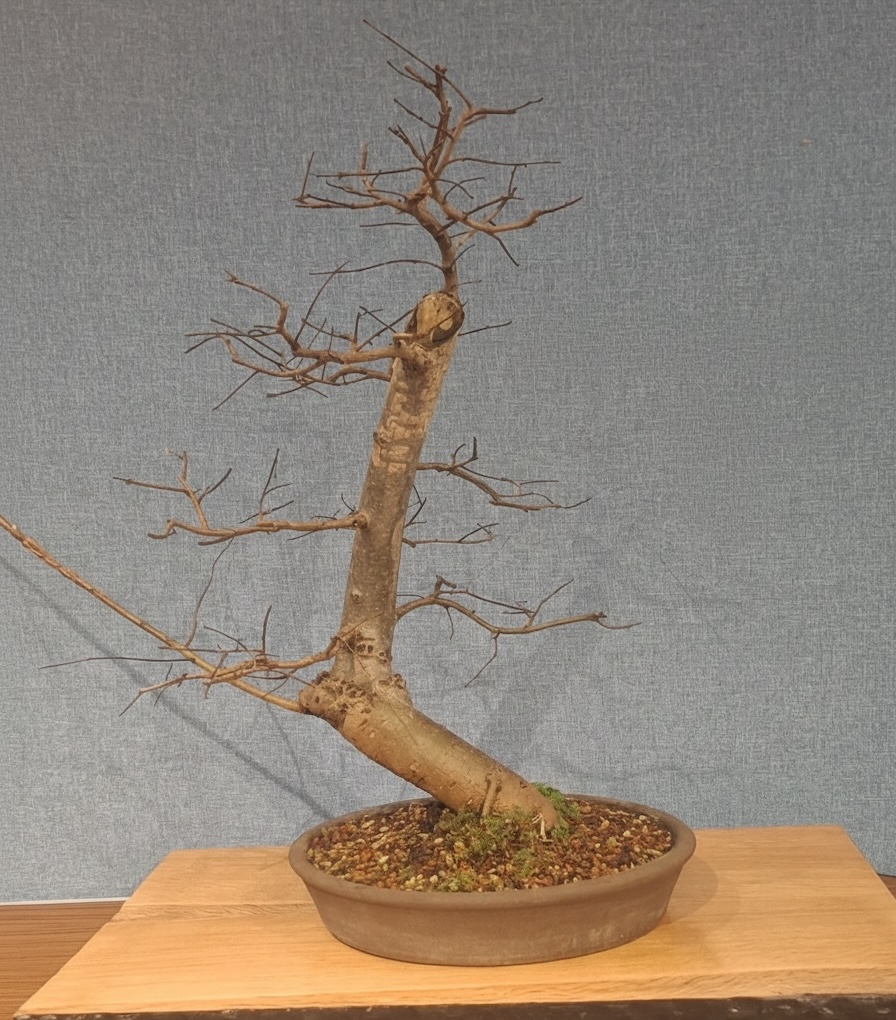
\includegraphics[angle=0,origin=c,width=1.0\textwidth]{2026_01/res/2601_totm_6_pittman}
\centerline{\emph{Mark Pittman's Elm.}}
\end{minipage}
\medskip

\vfill
\textcolor{white}{space}

\begin{minipage}[b]{.45\textwidth}
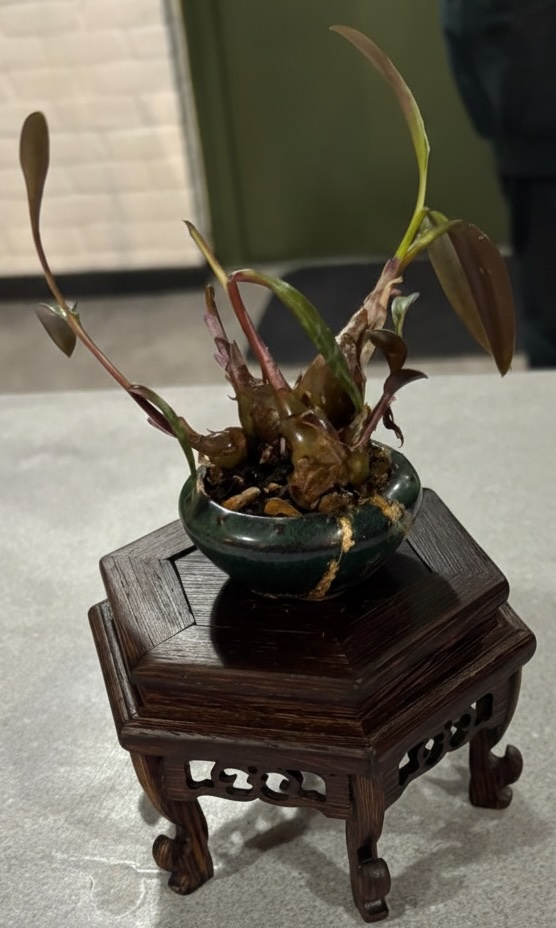
\includegraphics[angle=0,origin=c,width=1.0\textwidth]{2026_01/res/2601_totm_nov_laura}
\centerline{\emph{Laura Shantonas's Ledebouria.}}
\end{minipage}
\medskip

\vfill
\columnbreak
\clearpage
